% Created by tikzDevice version 0.12.6 on 2026-07-03 11:54:52
% !TEX encoding = UTF-8 Unicode
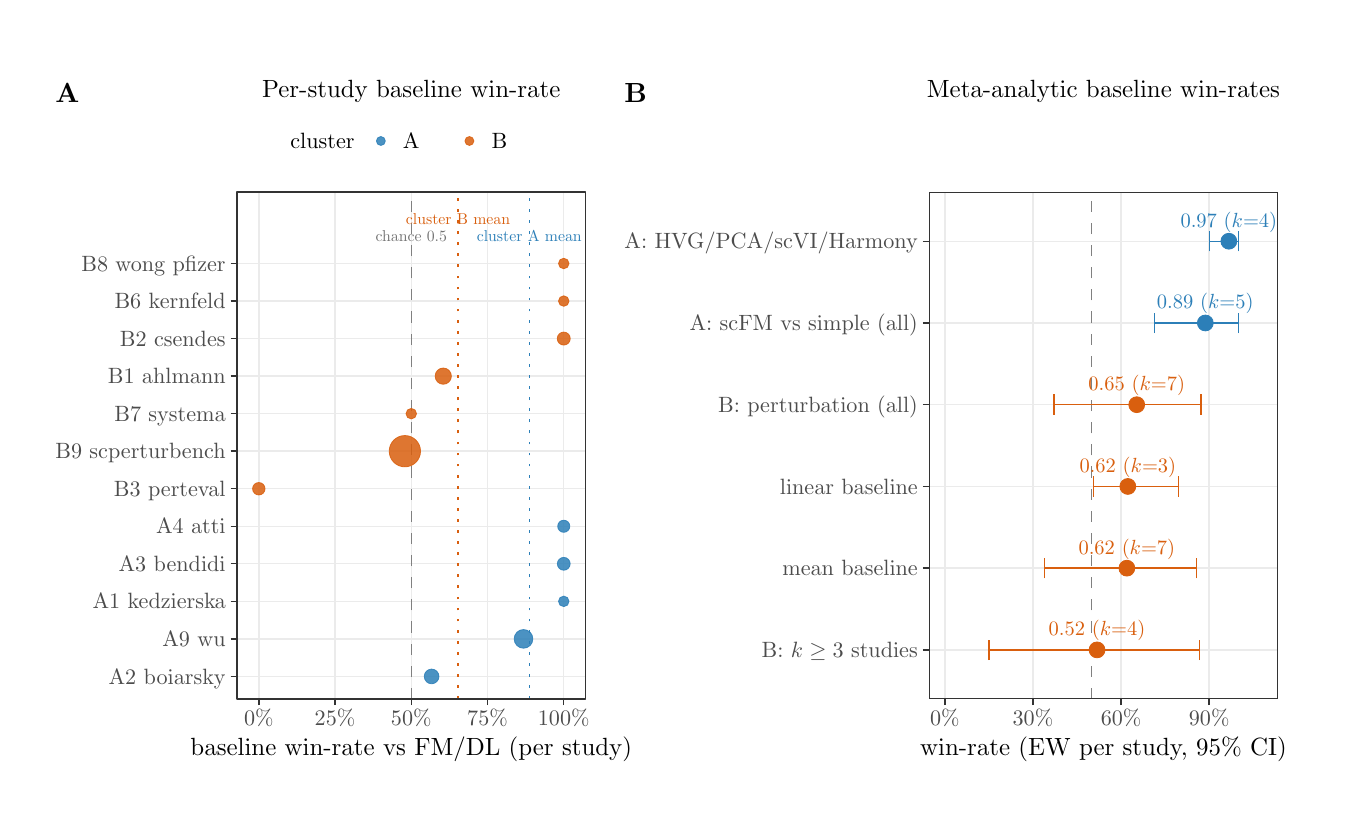
\begin{tikzpicture}[x=1pt,y=1pt]
\definecolor{fillColor}{RGB}{255,255,255}
\path[use as bounding box,fill=fillColor,fill opacity=0.00] (0,0) rectangle (469.75,274.63);
\begin{scope}
\path[clip] (  0.00,  0.00) rectangle (469.75,274.63);
\definecolor{drawColor}{RGB}{255,255,255}
\definecolor{fillColor}{RGB}{255,255,255}

\path[draw=drawColor,line width= 0.5pt,line join=round,line cap=round,fill=fillColor] (  0.00,  0.00) rectangle (469.75,274.63);
\end{scope}
\begin{scope}
\path[clip] (  5.00,  5.00) rectangle (210.64,269.63);
\definecolor{drawColor}{RGB}{255,255,255}
\definecolor{fillColor}{RGB}{255,255,255}

\path[draw=drawColor,line width= 0.5pt,line join=round,line cap=round,fill=fillColor] (  5.00,  5.00) rectangle (210.64,269.63);
\end{scope}
\begin{scope}
\path[clip] (210.64,  5.00) rectangle (460.75,269.63);
\definecolor{drawColor}{RGB}{255,255,255}
\definecolor{fillColor}{RGB}{255,255,255}

\path[draw=drawColor,line width= 0.5pt,line join=round,line cap=round,fill=fillColor] (210.64,  5.00) rectangle (460.75,269.63);
\end{scope}
\begin{scope}
\path[clip] (  0.00,  0.00) rectangle (469.75,274.63);
\definecolor{fillColor}{RGB}{255,255,255}

\path[fill=fillColor] ( 75.58, 32.07) rectangle (201.64,215.18);
\definecolor{drawColor}{gray}{0.92}

\path[draw=drawColor,line width= 0.5pt,line join=round] ( 75.58, 40.20) --
	(201.64, 40.20);

\path[draw=drawColor,line width= 0.5pt,line join=round] ( 75.58, 53.77) --
	(201.64, 53.77);

\path[draw=drawColor,line width= 0.5pt,line join=round] ( 75.58, 67.33) --
	(201.64, 67.33);

\path[draw=drawColor,line width= 0.5pt,line join=round] ( 75.58, 80.90) --
	(201.64, 80.90);

\path[draw=drawColor,line width= 0.5pt,line join=round] ( 75.58, 94.46) --
	(201.64, 94.46);

\path[draw=drawColor,line width= 0.5pt,line join=round] ( 75.58,108.02) --
	(201.64,108.02);

\path[draw=drawColor,line width= 0.5pt,line join=round] ( 75.58,121.59) --
	(201.64,121.59);

\path[draw=drawColor,line width= 0.5pt,line join=round] ( 75.58,135.15) --
	(201.64,135.15);

\path[draw=drawColor,line width= 0.5pt,line join=round] ( 75.58,148.71) --
	(201.64,148.71);

\path[draw=drawColor,line width= 0.5pt,line join=round] ( 75.58,162.28) --
	(201.64,162.28);

\path[draw=drawColor,line width= 0.5pt,line join=round] ( 75.58,175.84) --
	(201.64,175.84);

\path[draw=drawColor,line width= 0.5pt,line join=round] ( 75.58,189.41) --
	(201.64,189.41);

\path[draw=drawColor,line width= 0.5pt,line join=round] ( 83.52, 32.07) --
	( 83.52,215.18);

\path[draw=drawColor,line width= 0.5pt,line join=round] (111.06, 32.07) --
	(111.06,215.18);

\path[draw=drawColor,line width= 0.5pt,line join=round] (138.61, 32.07) --
	(138.61,215.18);

\path[draw=drawColor,line width= 0.5pt,line join=round] (166.16, 32.07) --
	(166.16,215.18);

\path[draw=drawColor,line width= 0.5pt,line join=round] (193.71, 32.07) --
	(193.71,215.18);
\definecolor{drawColor}{gray}{0.50}

\path[draw=drawColor,line width= 0.5pt,dash pattern=on 4pt off 4pt ,line join=round] (138.61, 32.07) -- (138.61,215.18);
\definecolor{drawColor}{RGB}{44,127,184}

\path[draw=drawColor,line width= 0.5pt,dash pattern=on 1pt off 3pt ,line join=round] (181.24, 32.07) -- (181.24,215.18);
\definecolor{drawColor}{RGB}{217,95,14}

\path[draw=drawColor,line width= 0.5pt,dash pattern=on 1pt off 3pt ,line join=round] (155.50, 32.07) -- (155.50,215.18);
\definecolor{drawColor}{gray}{0.45}

\node[text=drawColor,anchor=base,inner sep=0pt, outer sep=0pt, scale=  0.57] at (138.61,197.25) {chance 0.5};
\definecolor{drawColor}{RGB}{44,127,184}

\node[text=drawColor,anchor=base,inner sep=0pt, outer sep=0pt, scale=  0.57] at (181.24,197.25) {cluster A mean};
\definecolor{drawColor}{RGB}{217,95,14}

\node[text=drawColor,anchor=base,inner sep=0pt, outer sep=0pt, scale=  0.57] at (155.50,203.52) {cluster B mean};
\definecolor{drawColor}{RGB}{44,127,184}
\definecolor{fillColor}{RGB}{44,127,184}

\path[draw=drawColor,draw opacity=0.85,line width= 0.3pt,line join=round,line cap=round,fill=fillColor,fill opacity=0.85] (193.71, 67.33) circle (  1.90);

\path[draw=drawColor,draw opacity=0.85,line width= 0.3pt,line join=round,line cap=round,fill=fillColor,fill opacity=0.85] (145.96, 40.20) circle (  2.65);

\path[draw=drawColor,draw opacity=0.85,line width= 0.3pt,line join=round,line cap=round,fill=fillColor,fill opacity=0.85] (193.71, 80.90) circle (  2.31);

\path[draw=drawColor,draw opacity=0.85,line width= 0.3pt,line join=round,line cap=round,fill=fillColor,fill opacity=0.85] (193.71, 94.46) circle (  2.18);

\path[draw=drawColor,draw opacity=0.85,line width= 0.3pt,line join=round,line cap=round,fill=fillColor,fill opacity=0.85] (179.17, 53.77) circle (  3.37);
\definecolor{drawColor}{RGB}{217,95,14}
\definecolor{fillColor}{RGB}{217,95,14}

\path[draw=drawColor,draw opacity=0.85,line width= 0.3pt,line join=round,line cap=round,fill=fillColor,fill opacity=0.85] (150.17,148.71) circle (  2.93);

\path[draw=drawColor,draw opacity=0.85,line width= 0.3pt,line join=round,line cap=round,fill=fillColor,fill opacity=0.85] (193.71,162.28) circle (  2.34);

\path[draw=drawColor,draw opacity=0.85,line width= 0.3pt,line join=round,line cap=round,fill=fillColor,fill opacity=0.85] ( 83.52,108.02) circle (  2.24);

\path[draw=drawColor,draw opacity=0.85,line width= 0.3pt,line join=round,line cap=round,fill=fillColor,fill opacity=0.85] (193.71,175.84) circle (  1.90);

\path[draw=drawColor,draw opacity=0.85,line width= 0.3pt,line join=round,line cap=round,fill=fillColor,fill opacity=0.85] (138.61,135.15) circle (  1.90);

\path[draw=drawColor,draw opacity=0.85,line width= 0.3pt,line join=round,line cap=round,fill=fillColor,fill opacity=0.85] (193.71,189.41) circle (  1.90);

\path[draw=drawColor,draw opacity=0.85,line width= 0.3pt,line join=round,line cap=round,fill=fillColor,fill opacity=0.85] (136.30,121.59) circle (  5.65);
\definecolor{drawColor}{gray}{0.20}

\path[draw=drawColor,line width= 0.5pt,line join=round,line cap=round] ( 75.58, 32.07) rectangle (201.64,215.18);
\end{scope}
\begin{scope}
\path[clip] (  0.00,  0.00) rectangle (469.75,274.63);
\definecolor{drawColor}{gray}{0.30}

\node[text=drawColor,anchor=base east,inner sep=0pt, outer sep=0pt, scale=  0.80] at ( 71.53, 37.45) {A2 boiarsky};

\node[text=drawColor,anchor=base east,inner sep=0pt, outer sep=0pt, scale=  0.80] at ( 71.53, 51.01) {A9 wu};

\node[text=drawColor,anchor=base east,inner sep=0pt, outer sep=0pt, scale=  0.80] at ( 71.53, 64.58) {A1 kedzierska};

\node[text=drawColor,anchor=base east,inner sep=0pt, outer sep=0pt, scale=  0.80] at ( 71.53, 78.14) {A3 bendidi};

\node[text=drawColor,anchor=base east,inner sep=0pt, outer sep=0pt, scale=  0.80] at ( 71.53, 91.70) {A4 atti};

\node[text=drawColor,anchor=base east,inner sep=0pt, outer sep=0pt, scale=  0.80] at ( 71.53,105.27) {B3 perteval};

\node[text=drawColor,anchor=base east,inner sep=0pt, outer sep=0pt, scale=  0.80] at ( 71.53,118.83) {B9 scperturbench};

\node[text=drawColor,anchor=base east,inner sep=0pt, outer sep=0pt, scale=  0.80] at ( 71.53,132.39) {B7 systema};

\node[text=drawColor,anchor=base east,inner sep=0pt, outer sep=0pt, scale=  0.80] at ( 71.53,145.96) {B1 ahlmann};

\node[text=drawColor,anchor=base east,inner sep=0pt, outer sep=0pt, scale=  0.80] at ( 71.53,159.52) {B2 csendes};

\node[text=drawColor,anchor=base east,inner sep=0pt, outer sep=0pt, scale=  0.80] at ( 71.53,173.09) {B6 kernfeld};

\node[text=drawColor,anchor=base east,inner sep=0pt, outer sep=0pt, scale=  0.80] at ( 71.53,186.65) {B8 wong pfizer};
\end{scope}
\begin{scope}
\path[clip] (  0.00,  0.00) rectangle (469.75,274.63);
\definecolor{drawColor}{gray}{0.20}

\path[draw=drawColor,line width= 0.5pt,line join=round] ( 73.33, 40.20) --
	( 75.58, 40.20);

\path[draw=drawColor,line width= 0.5pt,line join=round] ( 73.33, 53.77) --
	( 75.58, 53.77);

\path[draw=drawColor,line width= 0.5pt,line join=round] ( 73.33, 67.33) --
	( 75.58, 67.33);

\path[draw=drawColor,line width= 0.5pt,line join=round] ( 73.33, 80.90) --
	( 75.58, 80.90);

\path[draw=drawColor,line width= 0.5pt,line join=round] ( 73.33, 94.46) --
	( 75.58, 94.46);

\path[draw=drawColor,line width= 0.5pt,line join=round] ( 73.33,108.02) --
	( 75.58,108.02);

\path[draw=drawColor,line width= 0.5pt,line join=round] ( 73.33,121.59) --
	( 75.58,121.59);

\path[draw=drawColor,line width= 0.5pt,line join=round] ( 73.33,135.15) --
	( 75.58,135.15);

\path[draw=drawColor,line width= 0.5pt,line join=round] ( 73.33,148.71) --
	( 75.58,148.71);

\path[draw=drawColor,line width= 0.5pt,line join=round] ( 73.33,162.28) --
	( 75.58,162.28);

\path[draw=drawColor,line width= 0.5pt,line join=round] ( 73.33,175.84) --
	( 75.58,175.84);

\path[draw=drawColor,line width= 0.5pt,line join=round] ( 73.33,189.41) --
	( 75.58,189.41);
\end{scope}
\begin{scope}
\path[clip] (  0.00,  0.00) rectangle (469.75,274.63);
\definecolor{drawColor}{gray}{0.20}

\path[draw=drawColor,line width= 0.5pt,line join=round] ( 83.52, 29.82) --
	( 83.52, 32.07);

\path[draw=drawColor,line width= 0.5pt,line join=round] (111.06, 29.82) --
	(111.06, 32.07);

\path[draw=drawColor,line width= 0.5pt,line join=round] (138.61, 29.82) --
	(138.61, 32.07);

\path[draw=drawColor,line width= 0.5pt,line join=round] (166.16, 29.82) --
	(166.16, 32.07);

\path[draw=drawColor,line width= 0.5pt,line join=round] (193.71, 29.82) --
	(193.71, 32.07);
\end{scope}
\begin{scope}
\path[clip] (  0.00,  0.00) rectangle (469.75,274.63);
\definecolor{drawColor}{gray}{0.30}

\node[text=drawColor,anchor=base,inner sep=0pt, outer sep=0pt, scale=  0.80] at ( 83.52, 22.51) {0\%};

\node[text=drawColor,anchor=base,inner sep=0pt, outer sep=0pt, scale=  0.80] at (111.06, 22.51) {25\%};

\node[text=drawColor,anchor=base,inner sep=0pt, outer sep=0pt, scale=  0.80] at (138.61, 22.51) {50\%};

\node[text=drawColor,anchor=base,inner sep=0pt, outer sep=0pt, scale=  0.80] at (166.16, 22.51) {75\%};

\node[text=drawColor,anchor=base,inner sep=0pt, outer sep=0pt, scale=  0.80] at (193.71, 22.51) {100\%};
\end{scope}
\begin{scope}
\path[clip] (  0.00,  0.00) rectangle (469.75,274.63);
\definecolor{drawColor}{RGB}{0,0,0}

\node[text=drawColor,anchor=base,inner sep=0pt, outer sep=0pt, scale=  0.90] at (138.61, 11.75) {baseline win-rate vs FM/DL (per study)};
\end{scope}
\begin{scope}
\path[clip] (  0.00,  0.00) rectangle (469.75,274.63);
\definecolor{fillColor}{RGB}{255,255,255}

\path[fill=fillColor] ( 90.44,224.18) rectangle (186.78,243.18);
\end{scope}
\begin{scope}
\path[clip] (  0.00,  0.00) rectangle (469.75,274.63);
\definecolor{drawColor}{RGB}{0,0,0}

\node[text=drawColor,anchor=base west,inner sep=0pt, outer sep=0pt, scale=  0.80] at ( 94.94,230.92) {cluster};
\end{scope}
\begin{scope}
\path[clip] (  0.00,  0.00) rectangle (469.75,274.63);
\definecolor{fillColor}{RGB}{255,255,255}

\path[fill=fillColor] (122.62,228.68) rectangle (132.62,238.68);
\definecolor{drawColor}{RGB}{44,127,184}
\definecolor{fillColor}{RGB}{44,127,184}

\path[draw=drawColor,draw opacity=0.85,line width= 0.3pt,line join=round,line cap=round,fill=fillColor,fill opacity=0.85] (127.62,233.68) circle (  1.61);
\end{scope}
\begin{scope}
\path[clip] (  0.00,  0.00) rectangle (469.75,274.63);
\definecolor{fillColor}{RGB}{255,255,255}

\path[fill=fillColor] (154.62,228.68) rectangle (164.62,238.68);
\definecolor{drawColor}{RGB}{217,95,14}
\definecolor{fillColor}{RGB}{217,95,14}

\path[draw=drawColor,draw opacity=0.85,line width= 0.3pt,line join=round,line cap=round,fill=fillColor,fill opacity=0.85] (159.62,233.68) circle (  1.61);
\end{scope}
\begin{scope}
\path[clip] (  0.00,  0.00) rectangle (469.75,274.63);
\definecolor{drawColor}{RGB}{0,0,0}

\node[text=drawColor,anchor=base west,inner sep=0pt, outer sep=0pt, scale=  0.80] at (135.62,230.92) {A};
\end{scope}
\begin{scope}
\path[clip] (  0.00,  0.00) rectangle (469.75,274.63);
\definecolor{drawColor}{RGB}{0,0,0}

\node[text=drawColor,anchor=base west,inner sep=0pt, outer sep=0pt, scale=  0.80] at (167.62,230.92) {B};
\end{scope}
\begin{scope}
\path[clip] (  0.00,  0.00) rectangle (469.75,274.63);
\definecolor{drawColor}{RGB}{0,0,0}

\node[text=drawColor,anchor=base,inner sep=0pt, outer sep=0pt, scale=  0.90] at (138.61,249.43) {Per-study baseline win-rate};
\end{scope}
\begin{scope}
\path[clip] (  0.00,  0.00) rectangle (469.75,274.63);
\definecolor{drawColor}{RGB}{0,0,0}

\node[text=drawColor,anchor=base,inner sep=0pt, outer sep=0pt, scale=  1.00] at ( 14.35,247.66) {\bfseries A};
\end{scope}
\begin{scope}
\path[clip] (325.70, 32.07) rectangle (451.75,215.18);
\definecolor{fillColor}{RGB}{255,255,255}

\path[fill=fillColor] (325.70, 32.07) rectangle (451.75,215.18);
\definecolor{drawColor}{gray}{0.92}

\path[draw=drawColor,line width= 0.5pt,line join=round] (325.70, 49.79) --
	(451.75, 49.79);

\path[draw=drawColor,line width= 0.5pt,line join=round] (325.70, 79.32) --
	(451.75, 79.32);

\path[draw=drawColor,line width= 0.5pt,line join=round] (325.70,108.85) --
	(451.75,108.85);

\path[draw=drawColor,line width= 0.5pt,line join=round] (325.70,138.39) --
	(451.75,138.39);

\path[draw=drawColor,line width= 0.5pt,line join=round] (325.70,167.92) --
	(451.75,167.92);

\path[draw=drawColor,line width= 0.5pt,line join=round] (325.70,197.46) --
	(451.75,197.46);

\path[draw=drawColor,line width= 0.5pt,line join=round] (331.43, 32.07) --
	(331.43,215.18);

\path[draw=drawColor,line width= 0.5pt,line join=round] (363.26, 32.07) --
	(363.26,215.18);

\path[draw=drawColor,line width= 0.5pt,line join=round] (395.09, 32.07) --
	(395.09,215.18);

\path[draw=drawColor,line width= 0.5pt,line join=round] (426.93, 32.07) --
	(426.93,215.18);
\definecolor{drawColor}{gray}{0.50}

\path[draw=drawColor,line width= 0.5pt,dash pattern=on 4pt off 4pt ,line join=round] (384.48, 32.07) -- (384.48,215.18);
\definecolor{drawColor}{RGB}{44,127,184}

\path[draw=drawColor,line width= 0.5pt,line join=round] (437.54,164.23) --
	(437.54,171.61);

\path[draw=drawColor,line width= 0.5pt,line join=round] (437.54,167.92) --
	(407.15,167.92);

\path[draw=drawColor,line width= 0.5pt,line join=round] (407.15,164.23) --
	(407.15,171.61);
\definecolor{drawColor}{RGB}{217,95,14}

\path[draw=drawColor,line width= 0.5pt,line join=round] (423.99,134.70) --
	(423.99,142.08);

\path[draw=drawColor,line width= 0.5pt,line join=round] (423.99,138.39) --
	(370.89,138.39);

\path[draw=drawColor,line width= 0.5pt,line join=round] (370.89,134.70) --
	(370.89,142.08);

\path[draw=drawColor,line width= 0.5pt,line join=round] (423.47, 46.09) --
	(423.47, 53.48);

\path[draw=drawColor,line width= 0.5pt,line join=round] (423.47, 49.79) --
	(347.43, 49.79);

\path[draw=drawColor,line width= 0.5pt,line join=round] (347.43, 46.09) --
	(347.43, 53.48);

\path[draw=drawColor,line width= 0.5pt,line join=round] (422.37, 75.63) --
	(422.37, 83.01);

\path[draw=drawColor,line width= 0.5pt,line join=round] (422.37, 79.32) --
	(367.52, 79.32);

\path[draw=drawColor,line width= 0.5pt,line join=round] (367.52, 75.63) --
	(367.52, 83.01);

\path[draw=drawColor,line width= 0.5pt,line join=round] (415.84,105.16) --
	(415.84,112.55);

\path[draw=drawColor,line width= 0.5pt,line join=round] (415.84,108.85) --
	(385.24,108.85);

\path[draw=drawColor,line width= 0.5pt,line join=round] (385.24,105.16) --
	(385.24,112.55);
\definecolor{drawColor}{RGB}{44,127,184}

\path[draw=drawColor,line width= 0.5pt,line join=round] (437.54,193.76) --
	(437.54,201.15);

\path[draw=drawColor,line width= 0.5pt,line join=round] (437.54,197.46) --
	(427.03,197.46);

\path[draw=drawColor,line width= 0.5pt,line join=round] (427.03,193.76) --
	(427.03,201.15);
\definecolor{fillColor}{RGB}{44,127,184}

\path[draw=drawColor,line width= 0.3pt,line join=round,line cap=round,fill=fillColor] (425.54,167.92) circle (  2.86);
\definecolor{drawColor}{RGB}{217,95,14}
\definecolor{fillColor}{RGB}{217,95,14}

\path[draw=drawColor,line width= 0.3pt,line join=round,line cap=round,fill=fillColor] (400.75,138.39) circle (  2.86);

\path[draw=drawColor,line width= 0.3pt,line join=round,line cap=round,fill=fillColor] (386.41, 49.79) circle (  2.86);

\path[draw=drawColor,line width= 0.3pt,line join=round,line cap=round,fill=fillColor] (397.19, 79.32) circle (  2.86);

\path[draw=drawColor,line width= 0.3pt,line join=round,line cap=round,fill=fillColor] (397.54,108.85) circle (  2.86);
\definecolor{drawColor}{RGB}{44,127,184}
\definecolor{fillColor}{RGB}{44,127,184}

\path[draw=drawColor,line width= 0.3pt,line join=round,line cap=round,fill=fillColor] (434.04,197.46) circle (  2.86);

\node[text=drawColor,anchor=base,inner sep=0pt, outer sep=0pt, scale=  0.74] at (425.54,173.02) {0.89 ($k{=}5$)};
\definecolor{drawColor}{RGB}{217,95,14}

\node[text=drawColor,anchor=base,inner sep=0pt, outer sep=0pt, scale=  0.74] at (400.75,143.48) {0.65 ($k{=}7$)};

\node[text=drawColor,anchor=base,inner sep=0pt, outer sep=0pt, scale=  0.74] at (386.41, 54.88) {0.52 ($k{=}4$)};

\node[text=drawColor,anchor=base,inner sep=0pt, outer sep=0pt, scale=  0.74] at (397.19, 84.42) {0.62 ($k{=}7$)};

\node[text=drawColor,anchor=base,inner sep=0pt, outer sep=0pt, scale=  0.74] at (397.54,113.95) {0.62 ($k{=}3$)};
\definecolor{drawColor}{RGB}{44,127,184}

\node[text=drawColor,anchor=base,inner sep=0pt, outer sep=0pt, scale=  0.74] at (434.04,202.55) {0.97 ($k{=}4$)};
\definecolor{drawColor}{gray}{0.20}

\path[draw=drawColor,line width= 0.5pt,line join=round,line cap=round] (325.70, 32.07) rectangle (451.75,215.18);
\end{scope}
\begin{scope}
\path[clip] (  0.00,  0.00) rectangle (469.75,274.63);
\definecolor{drawColor}{gray}{0.30}

\node[text=drawColor,anchor=base east,inner sep=0pt, outer sep=0pt, scale=  0.80] at (321.65, 47.03) {B: $k\geq3$ studies};

\node[text=drawColor,anchor=base east,inner sep=0pt, outer sep=0pt, scale=  0.80] at (321.65, 76.56) {mean baseline};

\node[text=drawColor,anchor=base east,inner sep=0pt, outer sep=0pt, scale=  0.80] at (321.65,106.10) {linear baseline};

\node[text=drawColor,anchor=base east,inner sep=0pt, outer sep=0pt, scale=  0.80] at (321.65,135.63) {B: perturbation (all)};

\node[text=drawColor,anchor=base east,inner sep=0pt, outer sep=0pt, scale=  0.80] at (321.65,165.17) {A: scFM vs simple (all)};

\node[text=drawColor,anchor=base east,inner sep=0pt, outer sep=0pt, scale=  0.80] at (321.65,194.70) {A: HVG/PCA/scVI/Harmony};
\end{scope}
\begin{scope}
\path[clip] (  0.00,  0.00) rectangle (469.75,274.63);
\definecolor{drawColor}{gray}{0.20}

\path[draw=drawColor,line width= 0.5pt,line join=round] (323.45, 49.79) --
	(325.70, 49.79);

\path[draw=drawColor,line width= 0.5pt,line join=round] (323.45, 79.32) --
	(325.70, 79.32);

\path[draw=drawColor,line width= 0.5pt,line join=round] (323.45,108.85) --
	(325.70,108.85);

\path[draw=drawColor,line width= 0.5pt,line join=round] (323.45,138.39) --
	(325.70,138.39);

\path[draw=drawColor,line width= 0.5pt,line join=round] (323.45,167.92) --
	(325.70,167.92);

\path[draw=drawColor,line width= 0.5pt,line join=round] (323.45,197.46) --
	(325.70,197.46);
\end{scope}
\begin{scope}
\path[clip] (  0.00,  0.00) rectangle (469.75,274.63);
\definecolor{drawColor}{gray}{0.20}

\path[draw=drawColor,line width= 0.5pt,line join=round] (331.43, 29.82) --
	(331.43, 32.07);

\path[draw=drawColor,line width= 0.5pt,line join=round] (363.26, 29.82) --
	(363.26, 32.07);

\path[draw=drawColor,line width= 0.5pt,line join=round] (395.09, 29.82) --
	(395.09, 32.07);

\path[draw=drawColor,line width= 0.5pt,line join=round] (426.93, 29.82) --
	(426.93, 32.07);
\end{scope}
\begin{scope}
\path[clip] (  0.00,  0.00) rectangle (469.75,274.63);
\definecolor{drawColor}{gray}{0.30}

\node[text=drawColor,anchor=base,inner sep=0pt, outer sep=0pt, scale=  0.80] at (331.43, 22.51) {0\%};

\node[text=drawColor,anchor=base,inner sep=0pt, outer sep=0pt, scale=  0.80] at (363.26, 22.51) {30\%};

\node[text=drawColor,anchor=base,inner sep=0pt, outer sep=0pt, scale=  0.80] at (395.09, 22.51) {60\%};

\node[text=drawColor,anchor=base,inner sep=0pt, outer sep=0pt, scale=  0.80] at (426.93, 22.51) {90\%};
\end{scope}
\begin{scope}
\path[clip] (  0.00,  0.00) rectangle (469.75,274.63);
\definecolor{drawColor}{RGB}{0,0,0}

\node[text=drawColor,anchor=base,inner sep=0pt, outer sep=0pt, scale=  0.90] at (388.73, 11.75) {win-rate (EW per study, 95\% CI)};
\end{scope}
\begin{scope}
\path[clip] (  0.00,  0.00) rectangle (469.75,274.63);
\definecolor{drawColor}{RGB}{0,0,0}

\node[text=drawColor,anchor=base,inner sep=0pt, outer sep=0pt, scale=  0.90] at (388.73,249.43) {Meta-analytic baseline win-rates};
\end{scope}
\begin{scope}
\path[clip] (  0.00,  0.00) rectangle (469.75,274.63);
\definecolor{drawColor}{RGB}{0,0,0}

\node[text=drawColor,anchor=base,inner sep=0pt, outer sep=0pt, scale=  1.00] at (219.73,247.66) {\bfseries B};
\end{scope}
\end{tikzpicture}
